%
% exemplo genérico de uso da classe iiufrgs.cls
% $Id: iiufrgs.tex,v 1.1.1.1 2005/01/18 23:54:42 avila Exp $
%
% This is an example file and is hereby explicitly put in the
% public domain.
%
\documentclass[ppgc,mestrado,biblatex]{iiufrgs}
% um tipo específico de monografia pode ser informado como parâmetro opcional:
%\documentclass[ppgc,tese,biblatex]{iiufrgs}
% monografias em inglês devem receber o parâmetro `english':
%\documentclass[ppgc,diss,english,biblatex]{iiufrgs}
% a opção `openright' pode ser usada para forçar inícios de capítulos
% em páginas ímpares
% \documentclass[ppgc,mestrado,openright,biblatex]{iiufrgs}
% para gerar uma versão somente-frente, basta utilizar a opção `oneside':
% \documentclass[ppgc,mestrado,oneside,biblatex]{iiufrgs}
% para utilizar o pacote legado abntex2cite (com bibtex) em vez de biblatex:
% \documentclass[ppgc,mestrado,abntex2cite]{iiufrgs}

\addbibresource{biblio.bib}

% Pacotes recomendados para recursos adicionais
\usepackage{booktabs}        % Tabelas profissionais com linhas abertas (\toprule, \midrule, \bottomrule)
\usepackage{amsmath,amssymb} % Símbolos e equações matemáticas
\usepackage{listings}        % Listagens de código-fonte
\usepackage{microtype}       % Ajuste tipográfico fino de margens e caracteres

% Configuração padrão para trechos de código (listings)
\lstset{
    basicstyle=\ttfamily\small,
    keywordstyle=\bfseries,
    numbers=none,
    frame=single,
    breaklines=true,
    captionpos=t,
    tabsize=2,
    showstringspaces=false
}

%
% Informações gerais
%
\title{Um Exemplo de Monografia do Instituto de Informática da UFRGS}
\translatedtitle{Using \LaTeX\ to Prepare Documents at II/UFRGS}

\author{Flaumann}{Fritz Gutenberg}
% alguns documentos podem ter varios autores:
%\author{Flaumann}{Frida Gutenberg}
%\author{Flaumann}{Klaus Gutenberg}

% orientador e co-orientador são opcionais (não diga isso pra eles :))
\advisor[Prof.~Dr.]{Lamport}{Leslie}
%\coadvisor[Prof.~Dr.]{Knuth}{Donald Ervin}

% a data deve ser a da defesa; se nao especificada, são gerados
% mes e ano correntes
%\date{maio}{2001}

% o nome do curso pode ser redefinido (ex. para TCs)
%\course{Curso de Especialização em Cachaça}

% o local de realização do trabalho pode ser especificado (ex. para TCs)
% com o comando \location:
%\location{Porto Alegre}{RS}

% ------------------------------------------------------------------------------
% Nominata Institucional (Personalização Dinâmica de Gestão)
% ------------------------------------------------------------------------------
% Os cargos da administração (Reitora, Pró-Reitor, Diretor do II, Coordenador etc.)
% são definidos centralizadamente em `nominata.def` e associados dinamicamente ao curso
% escolhido (`ppgc.def`, `cic.def`, etc.).
% Caso ocorram alterações em cargos de gestão, você pode:
%   a) Atualizar diretamente o arquivo `nominata.def`;
%   b) Ou redefinir comandos específicos aqui no preâmbulo com \renewcommand:
%      \renewcommand{\nominataCoord}{Prof.~Nome Sobrenome}
%      \renewcommand{\nominataCoordname}{Coordenador do PPGC}
%      \renewcommand{\nominataDir}{Prof.~Nome Sobrenome}
%      \renewcommand{\nominataReit}{Prof\textsuperscript{a}.~Nome Sobrenome}
%   c) Ou criar um arquivo `nominatalocal.def` e passar a opção [nominatalocal] na classe.
% ------------------------------------------------------------------------------

% A seguir são apresentados comandos específicos para alguns
% tipos de documentos.

% Relatório de Pesquisa [rp]:
% \rp{123}             % numero do rp
% \financ{CNPq, CAPES} % orgaos financiadores

% Trabalho Individual [ti]:
% \ti{123}     % numero do TI
% \ti[II]{456} % no caso de ser o segundo TI

% Trabalho de Conclusão [tc]:
% além de definir explicitamente o nome do curso (\course) e o local
% de realização (\location), é necessário redefinir a nominata,
% pois as informações necessárias dependem do curso. Ex.:
%\renewcommand{\nominata}{
%        UNIVERSIDADE FEDERAL DO RIO GRANDE DO SUL\\
%        Reitora: Prof\textsuperscript{a}.~Wrana Maria Panizzi\\
%        Pró-Reitor de Ensino: Prof.~José Carlos Ferraz Hennemann\\
%        Diretor do Instituto de Informática: Prof.~Philippe Olivier Alexandre Navaux\\
%        Coordenador do curso: Prof.~Seu Creysson\\
%        Bibliotecária-chefe do Instituto de Informática: Beatriz Regina Bastos Haro
%}

% Monografias de Especialização [espec]:
% \espec{Redes e Sistemas Distribuídos}      % nome do curso
% \coord[Profa.~Dra.]{Weber}{Taisy da Silva} % coordenador do curso
% \dept{INA}                                 % departamento relacionado

%
% palavras-chave
% iniciar todas com letras maiúsculas
%
\keyword{Formatação eletrônica de documentos}
\keyword{\LaTeX}
\keyword{ABNT}
\keyword{UFRGS}

%
% palavras-chave na lingua estrangeira
% iniciar todas com letras maiúsculas
%
\translatedkeyword{Electronic document preparation}
\translatedkeyword{\LaTeX}
\translatedkeyword{ABNT}
\translatedkeyword{UFRGS}

%
% inicio do documento
%
\begin{document}

% folha de rosto
% às vezes é necessário redefinir algum comando logo antes de produzir
% a folha de rosto:
% \renewcommand{\coordname}{Coordenadora do Curso}
\maketitle

% dedicatoria
\begin{dedicatoria}
\textit{``If I have seen farther than others,\\
it is because I stood on the shoulders of giants.''\\}
--- \textsc{Sir~Isaac Newton}
\end{dedicatoria}

% agradecimentos
\begin{agradecimentos}
Agradeço ao \LaTeX\ por sua solidez e precisão tipográfica, ao Instituto de Informática e a todos os professores e colegas que tornaram este trabalho possível.
\end{agradecimentos}

% resumo na língua do documento
\begin{abstract}
Este documento é um exemplo de como formatar documentos para o
Instituto de Informática da UFRGS usando as classes \LaTeX\
disponibilizadas pelo UTUG\@. Ao mesmo tempo, pode servir de consulta
para comandos mais genéricos. \emph{O texto do resumo não deve
conter mais do que 500 palavras.}
\end{abstract}

% resumo na outra língua
\begin{translatedabstract}
This document is an example on how to prepare documents at II/UFRGS
using the \LaTeX\ classes provided by the UTUG\@. At the same time, it
may serve as a guide for general-purpose commands. \emph{The text in
the abstract should not contain more than 500~words.}
\end{translatedabstract}

% lista de abreviaturas e siglas
% o parametro deve ser a abreviatura mais longa
% A NBR 14724 estipula que a ordem das abreviações
% na lista deve ser alfabética (como no exemplo abaixo).
\begin{listofabbrv}{SPMD}
        \item[ABNT] Associação Brasileira de Normas Técnicas
        \item[NUMA] Non-Uniform Memory Access
        \item[SIMD] Single Instruction Multiple Data
        \item[SMP] Symmetric Multi-Processor
        \item[SPMD] Single Program Multiple Data
\end{listofabbrv}

% idem para a lista de símbolos
%\begin{listofsymbols}{$\alpha\beta\pi\omega$}
%       \item[$\sum{\frac{a}{b}}$] Somatório do produtório
%       \item[$\alpha\beta\pi\omega$] Fator de inconstância do resultado
%\end{listofsymbols}

% lista de figuras
\listoffigures

% lista de tabelas
%\listoftables

% sumario (último elemento pré-textual conforme ABNT NBR 14724)
\tableofcontents

% aqui comeca o texto propriamente dito

% introducao
\chapter{Introdução}
No início dos tempos, Donald E. Knuth criou o \TeX. Algum tempo depois, Leslie Lamport criou o \LaTeX. Graças a eles, não somos obrigados a usar o Word nem o StarOffice.

\section{Figuras e Tabelas segundo as Normas ABNT e IBGE}

Esta seção faz referência às Figuras~\ref{fig:ex1},~\ref{fig:ex2} e~\ref{fig:ex_nodes}, bem como às Tabelas~\ref{tbl:ex1} e~\ref{tbl:ex_externa}, a título de exemplo.

Conforme as normas do Instituto de Informática e da ABNT:
\begin{itemize}
    \item A identificação e o título (\texttt{\string\caption}) aparecem sempre \textbf{acima} do elemento ilustrativo;
    \item A indicação da autoria ou fonte (\texttt{\string\legend} ou \texttt{\string\fonte}) é \textbf{obrigatória} e deve figurar \textbf{abaixo}, inclusive em produções próprias (\emph{Fonte: O Autor} ou \emph{Fonte: Elaborada pelo autor});
    \item Ilustrações ou dados adaptados de terceiros devem indicar a referência e a \textbf{página exata} de origem.
\end{itemize}

A Figura~\ref{fig:ex1} representa o caso mais comum, no qual a figura é importada de um arquivo vetorial ou matricial (veja a Seção~\ref{sec:fig_format}). A Figura~\ref{fig:ex2} exemplifica o desenho esquemático com o ambiente \texttt{picture}. Já a Figura~\ref{fig:ex_nodes} exemplifica uma ilustração adaptada de outro autor.

\begin{figure}[htbp]
    \centering
    \caption{Exemplo de figura importada de um arquivo.}
    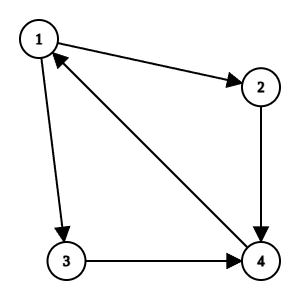
\includegraphics[width=0.3\linewidth]{figures/graph.png}
    \legend{Fonte: Elaborada pelo autor}
    \label{fig:ex1}
\end{figure}

\begin{figure}[htbp]
    \centering
    \caption{Exemplo de figura desenhada com o ambiente \texttt{picture}.}
    \setlength{\unitlength}{.1em}
    \begin{picture}(100,60)
        \put(20,20){\circle{20}}
        \put(20,20){\small\makebox(0,0){a}}
        \put(80,40){\circle{20}}
        \put(80,40){\small\makebox(0,0){b}}
        \put(28,24){\vector(3,1){44}}
    \end{picture}
    \legend{Fonte: Elaborada pelo autor}
    \label{fig:ex2}
\end{figure}

\begin{figure}[htbp]
    \centering
    \caption{Exemplo de figura adaptada de outro autor com indicação de página.}
    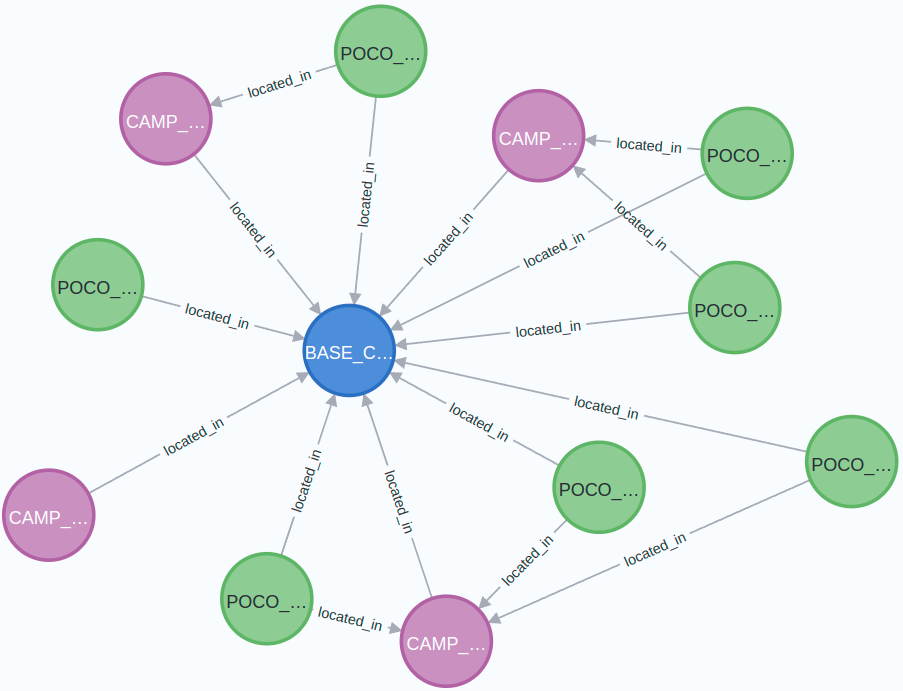
\includegraphics[width=0.7\linewidth]{figures/nodes.png}
    \legend{Fonte: Adaptada de \textcite[p.~10]{besta2023demystifying}}
    \label{fig:ex_nodes}
\end{figure}

\subsection{Construção de Tabelas segundo o Padrão IBGE/ABNT}

Conforme as normas de apresentação tabular do IBGE e da ABNT, as tabelas possuem bordas laterais \textbf{abertas} (sem grades verticais delimitadoras externas). Recomenda-se o uso do pacote \texttt{booktabs} com \texttt{\string\toprule}, \texttt{\string\midrule} e \texttt{\string\bottomrule}.

A Tabela~\ref{tbl:ex1} apresenta um exemplo de tabela de autoria própria, e a Tabela~\ref{tbl:ex_externa} ilustra dados adaptados de outro autor:

\begin{table}[htbp]
    \centering
    \caption{Exemplo de tabela de autoria própria.}
    \label{tbl:ex1}
    \begin{tabular}{ccp{7cm}}
        \toprule
        \textbf{Identificador} & \textbf{Estado} & \textbf{Descrição da Operação} \\
        \midrule
        OP\_01 & Concluída  & Processamento de indexação semântica de entidades. \\
        OP\_02 & Pendente   & Carga em lote de relacionamentos no banco de grafos. \\
        OP\_03 & Em Análise & Avaliação de coerência temporal de asserções. \\
        \bottomrule
    \end{tabular}
    \legend{Fonte: Elaborada pelo autor}
\end{table}

\begin{table}[htbp]
    \centering
    \caption{Comparação de características arquiteturais entre modelos de bancos de dados.}
    \label{tbl:ex_externa}
    \begin{tabular}{p{3.8cm}p{4.5cm}p{4.8cm}}
        \toprule
        \textbf{Critério de Análise} & \textbf{Bancos Relacionais (RDBMS)} & \textbf{Bancos em Grafos} \\
        \midrule
        Modelo de Dados & Tabelas normalizadas (linhas e colunas) & Nós, relacionamentos e propriedades \\
        Navegação entre Relações & Junções (\textit{JOINs}) computacionalmente caras & Travessia direta por ponteiros (\textit{index-free}) \\
        Desempenho com Saltos & Decai exponencialmente com a profundidade & Proporcional ao subgrafo explorado \\
        \bottomrule
    \end{tabular}
    \legend{Fonte: Adaptada de \textcite[p.~18]{vukotic2014neo4j}}
\end{table}

\subsection{Formatos de Figuras}
\label{sec:fig_format}

O \LaTeX\ permite utilizar vários formatos de imagens, destacando-se formatos vetoriais (\emph{pdf}, \emph{svg}) e matriciais de alta resolução (\emph{png}, \emph{jpeg}). Programas como Inkscape geram diagramas vetoriais em PDF que mantêm nitidez em qualquer aproximação.

\subsection{Níveis de Seções}

O formato adotado pela ABNT prevê apenas três níveis de subdivisão numerada (capítulo, seção e subseção). O uso de subdivisões mais profundas como \texttt{\string\subsubsection} não é aconselhado.

\section{Citações segundo a Norma ABNT NBR 10520}

A classe \emph{iiufrgs} integra-se nativamente ao \textsf{biblatex} com o estilo \textsf{abnt}. Conforme a ABNT NBR~10520, deve-se distinguir rigorosamente as seguintes modalidades de citação:

\subsection{Citação Indireta (Paráfrase)}
Reprodução livre das ideias do autor consultado com suas próprias palavras:
\begin{itemize}
    \item \textbf{No fluxo da frase (sistema autor-data em minúsculas)}:\\
    utiliza-se \texttt{\string\textcite\{chave\}} (ou os sinônimos legados \texttt{\string\citet} e \texttt{\string\citeonline}).\\
    \emph{Exemplo}: De acordo com \textcite{elmasri2005sistemas}, a modelagem conceitual de dados precede a modelagem lógica e física.
    
    \item \textbf{Ao final do período (entre parênteses em MAIÚSCULAS)}:\\
    utiliza-se \texttt{\string\cite\{chave\}} (ou \texttt{\string\parencite} / \texttt{\string\citep}):\\
    \emph{Exemplo}: A arquitetura Transformer revolucionou o processamento de linguagem natural moderna~\cite{vaswani2017attention}.
    
    \item \textbf{Apenas o ano}:\\
    utiliza-se \texttt{\string\citeyearpar\{chave\}} quando o autor já foi nomeado no texto.\\
    \emph{Exemplo}: Nos experimentos conduzidos por Vukotic et al.~\citeyearpar{vukotic2014neo4j}, analisou-se o custo computacional de junções.
\end{itemize}

\subsection{Citação Direta Curta (até 3 linhas)}
Transcrição textual literal das palavras do autor original. Deve ser inserida no próprio corpo do parágrafo, \textbf{obrigatoriamente entre aspas duplas} e com a indicação da \textbf{página exata} de origem:
\begin{itemize}
    \item \textbf{Exemplo}: Conforme sintetizam \textcite[p.~15]{Adams2009Conceptual}, ``\foreignlanguage{english}{the universe is not only stranger than we imagine, but stranger than we can imagine}''.
\end{itemize}

\subsection{Citação Direta Longa (mais de 3 linhas)}
Quando a citação textual exceder \textbf{três linhas}, deve ser apresentada em bloco isolado, com recuo de \textbf{4~cm} da margem esquerda, tamanho de fonte reduzido (\textbf{10~pontos}), espaçamento entrelinhas \textbf{simples}, sem aspas e com indicação formal de autor, ano e página. Para isso, utilize o ambiente \texttt{citacao} (ou \texttt{quote}):

\begin{citacao}
Um sistema de gerenciamento de banco de dados (SGBD) é uma coleção de programas que permite aos usuários criar e manter um banco de dados. O SGBD é um sistema de software de propósito geral que facilita os processos de definição, construção, manipulação e compartilhamento de bancos de dados entre vários usuários e aplicações~\cite[p.~4]{elmasri2005sistemas}.
\end{citacao}

\subsection{Citação de Citação (\textit{Apud})}
Utilizada quando se faz referência a um texto original ao qual o autor não teve acesso direto. Conforme a ABNT, deve-se usar a expressão latina em itálico \textit{apud}. No \textsf{biblatex-abnt}, pode-se utilizar o comando nativo:\\
\verb|\apud[p.~Y]{autor_original}{autor_secundario}|\\
ou formular textualmente a relação indicando a obra consultada. Recomenda-se evitar o \textit{apud} sempre que a fonte primária for acessível.

% e aqui vai a parte principal
%
% \chapter{Estado da arte}
% \chapter{Mais estado da arte}
% \chapter{A minha contribuição}
% \chapter{Prova de que a minha contribuição é válida}
% \chapter{Conclusão}

\printbibliography

\end{document}
